\documentclass[border=10pt]{standalone}
\usepackage{tikz}
\usetikzlibrary{calc}
\usetikzlibrary{arrows,positioning,shapes.geometric}
% for i in 1 2 3; do pdftoppm -png process_video$i.pdf > process_video$i.png; done
\begin{document}
    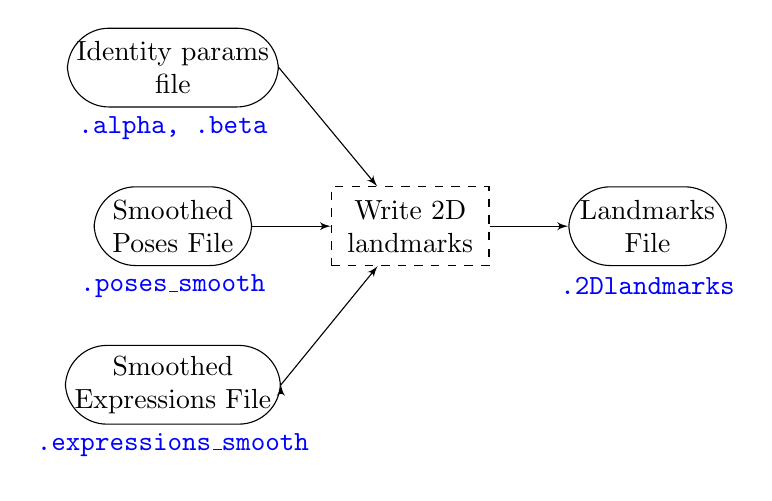
\begin{tikzpicture}[>=latex']
        \tikzset{block/.style= {draw, rectangle, align=center,minimum width=2cm,minimum height=1cm},
        dblock/.style= {draw=black,dashed,  align=center,minimum width=2cm,minimum height=1cm},
        int/.style={minimum size=2em,font=\ttfamily,text=blue},
        rblock/.style={draw, shape=rectangle,rounded corners=1.5em,align=center,minimum width=2cm,minimum height=1cm},
        input/.style={ % requires library shapes.geometric
        draw,
        trapezium,
        trapezium left angle=60,
        trapezium right angle=120,
        minimum width=2cm,
        align=center,
        minimum height=1cm
    },
        }
        
        \node [rblock] (poses) {Smoothed \\Poses File};
        \node [rblock,above=1cm of poses] (id) {Identity params \\file};
		\node [int, below=-0.1cm of id] (id_ext) {.alpha, .beta};

        \node [rblock, below=1cm of poses] (exps) {Smoothed\\Expressions File};
        
        \node [dblock, right=1cm of poses] (lmks) {Write 2D \\landmarks};
        \node [int, below=-0.1cm of poses] (poses_ext) {.poses\_smooth};
        \node [int, below=-0.1cm of exps] (exps_ext) {.expressions\_smooth};
        \node [rblock, right=1cm of lmks] (lmks_file) {Landmarks\\File};
        \node [int, below=-0.1cm of lmks_file] (lmks_ext) {.2Dlandmarks};

%%% paths
        \path[draw,->] (poses) edge (lmks)
        				(id.east) edge (lmks)
                    (exps.east) edge (lmks)
                    (lmks) edge (lmks_file)
                    ;
    \end{tikzpicture}
\end{document}